The presence of dust in space was hypothesized long ago by \citet{cassini1685} as an explanation for the faint light on the night sky near the plane of ecliptics. Dust was also observed locally, that is \textit{in-situ}, by its interaction with spacecraft since the dawn of the space age, when the concern about the risk it posed to the spacecraft was present \citep{whipple1958meteoritic}. This chapter provides an introduction into dust detection methods in general, and into antenna detected impact ionization in particular, since it is vital for the rest of the present work.

\section{Remote observations}

Since dust grains in space absorb light, they are observed by extinction of light, \citep{desert1990interstellar} allowing for transmission spectroscopy, which is useful on the galactic scale \citep{mann2010interstellar}. In terms of the Solar system, refraction, reflection, and thermal emission by dust is important, since it shows the spatial distribution and size distribution of dust in the zodiacal cloud \citep{allen1946spectrum,hulst1947zodiacal,leinert1981zodiacal,stenborg2018characterization,stenborg2021psp}. Measurements of luminance in principle integrate the luminosity on a line of sight (\textit{LOS}) between the observer and infinity. Most of the luminosity originates near the Sun, where both the dust density and the sunlight are the strongest. However, as the existence of Gegenschein shows \citep{roosen1971gegenschein}, scattering is very angle-dependent. It favors smaller angles and, therefore, the sources closer to the observer, and makes the inversion of LOS luminance into dust density more model dependent and ambiguous \citep{mann2004dust,kneissel1991spatial}. Observations from $\SI{1}{AU}$ are therefore limited, especially a few angular degrees from the Sun. The best results are achieved with measurements closer to the Sun, such as those of the two \textit{Helios} spacecraft \cite{leinert1981zodiacal}, which, as we mentioned in the previous chapter (Eq. \ref{eq:dust_number_density}), found the number density of bound dust between $\SI{0.3}{AU}$ and $\SI{1}{AU}$ scaling as $n(R) \propto R^{-1.3}$. More recently, measurements of the Wide-field Imager for Solar Probe (\textit{WISPR}) confirmed this trend \citep{stenborg2021psp}, and even observed a dust depletion zone \citep{stenborg2022psp}. The measurements are difficult to interpret because the luminance of dust-caused F-corona and dust-independent K-corona are hard to distinguish. 

WISPR observed many phenomena, one of them being the clouds of spacecraft debris liberated by impacts of hypervelocity dust on the insulating carbon foam \citep{malaspina2022clouds}. The carbon thermal insulation is fragile and the debris move slowly enough that the light they scatter is captured in individual shots, allowing for the estimation of their speed, which was found to be on the order of $\si{m s^{-1}}$. Trajectories of the debris were also found to be curved around biased electrical antennas, which is a motion similar to the motion of electrons in \citeauthor{pantellini2012nano} process \citep{pantellini2012nano}, which we hypothesize might be responsible for the double-peak signals reported on SolO in Paper III. 


\section{Impact ionization}

\subsection{Charge generation process}

A very fast impact of a dust grain onto a solid target, such as spacecraft body, releases free charges. This is because of the great energy density at the impact site \citep{shen2021cosmic}. At moderate relative speeds of $v \lesssim \SI{10}{kms^{-1}}$, the ionization is mostly due to surface effects on the grain and on the target \citep{kissel1987ion}. At much higher speeds $v \gtrsim \SI{20}{kms^{-1}}$, the grain is destroyed completely and the ionization is due to the effects in the bulk of the target \citep{hornung1994shock}. For this, shock wave formation in the target at supersonic speed is important \citep{drapatz1974theory}, which concentrates the available energy into the shock front, which makes up a small volume of the target, resulting in high volumetric energy density. 

The first reported observation \citep{friichtenicht1964} of impact ionization followed shortly after the development of the first $MV$ dust accelerator \citep{friichtenicht1962}. The charge leaving the impact site after the impact of carbon and iron dust grains was measured with a pre-amplifier connected to a metallic target. The charge was observed to be quasineutral, and the amount of generated charge $q$ was found consistent with the relation
\begin{equation}
    q \propto m v^3,
\end{equation}
for the velocities  $\SI{2}{kms^{-1}} < v < \SI{15}{kms^{-1}}$, where $m$ is the mass of the grain and $v$ is the impact speed. Later measurements \citep{auer1968,mcbride1999meteoroid,grun1984impact,collette2014micrometeoroid,shen2021cosmic} worked with a more general empirical equation of 
\begin{equation}
    q \propto m^\alpha v^\beta, \label{eq:charge_generation}
\end{equation}
and mostly found $\alpha \approx 1$ and $3 < \beta < 5$, depending on the speed interval and the combination of the grain material and the target material.

\subsection{Laboratory simulation}

The most successful dust accelerators are based on electrostatic acceleration principle, not dissimilar to the ion gun. The latest such device, operated at \textit{IMPACT}, offers the acceleration voltage of up to $\SI{3}{MV}$ \citep{shu20123}, allowing for speeds up to $v\gtrsim \SI{50}{kms^{-1}}$ for $r\lesssim\SI{1}{\mu m}$ grains, measuring both the mass and the charge state of the grain right before it hits the target. It not only allows for study of the impact ionization process \citep{shen2021electrostatic,shen2023variability,nouzak2018laboratory,nouzak2021detection,kovcivsvcak2020effective,collette2014micrometeoroid}, but also for the study of atmospheric ablation \citep{thomas2017experimental,deluca2018ionization,deluca2022differential,tarnecki2023experimentally}. Many aspects of each impact can be measured at the same time, as there is no payload or transmission capacity limitation, such as in the case of spacecraft experimens. Although versatile, accelerator measurements bear disadvantages: the experiment happens in a confined chamber in finite vacuum, the accelerated dust grain is selected randomly from a reservoir, and there is an intrinsic correlation between the speed and the mass of a grain, given the charge and the accelerating voltage are constant \citep{shelton1960electrostatic}. As far as the replication of space environment goes, the plasma conditions (solar wind, UV illumination) can be partially replicated in laboratory \citep{shu20123,horanyi2008surface}, but the noise level in laboratory is never as low as in space. 

\subsection{Dedicated ionization detectors}

The mechanism of impact ionization is used to detect dust impacts on spacecraft. In principle, a surface is located in a chamber, where the entry of charged particles is blocked by a filter, which is however not capable of blocking the entry of dust grains.  The surface is therefore exposed to potential dust impacts, which are the only thinkable source of charge in the chamber. Charge is monitored with a bias collector in the chamber, and whenever it appears, it is due to a dust impact. The first such detector was used on the \textit{OGO 3} mission \citep{alexander1968zodiacal}, and was used many times in forms of variable complexity, some of them resolving the charge and directionality \citep{grun1992galileo,grun1992ulysses,berg1969pioneer} of the incident grains, or even allowing for spectroscopy of the impact plasma \citep{srama2004cassini,sommer2023measuring}. Impact ionization detectors are very sensitive and versatile, and they are used not only in orbit, but also on sounding rockets \citep{gunnarsdottir2019charging,trollvik2019observation} to study smoke particles in the mesosphere. 

\subsection{Non-ionization dust detectors}

\subsubsection{Mechanical methods} 

A penetration method was employed on \textit{Pionner 10} and \textit{11} \citep{humes1980results}. A $\SI{25}{\mu m}$ and a $\SI{50}{\mu m}$ pressurized steel cells were mounted on \textit{Pionner 10} and \textit{11} respectively, $234$ cells on each, counting the impacts of dust grains fast and big enough to penetrate them, which showed by the pressure loss in the cell. Together, these detectors counted $182$ dust impacts, showing clearly higher abundance of dust near Jupiter and Saturn, and concluding that the $\approx \SI{10}{\mu m}$ grains observed between the asteroid belt and Jupiter were not circular and in the ecliptic plane, but rather eccentric or inclined. 

An integration experiment was conducted on the Long Duration Exposure Facility \textit{LDEF} satellite \citep{love1993direct}, which consisted of a study of $\SI{5.6}{m^2}$ aluminium plate exposed to the near Earth environment for nearly six years. In total $761$ craters were found on a microscope scan, allowing for the estimate of the total meteoric mass accretion rate by the Earth to $40 \pm 20 \, \si{kg y^{-1}}$. 

Aerogel, an extremely low-density silica material, was shown to provide gentle enough dissipation of kinetic energy to capture hypervelocity cosimc dust grains intact \citep{tsou1995silica}. The same material was used to recover a dust sample from the \textit{Wild 2} comet, which was achieved by the \textit{Stardust} mission \citep{brownlee2014stardust}. 

\subsubsection{Piezoelectric}

In the early age of in-situ dust science, dust was detected with so-called microphone detectors \citep{alexander1963review}. The principle is very simple, as such device consists of a hard target connected to a piezoelectric element, which acoustically registers each strong enough impact. The detectors were however often sensitive ot other effects, which led to vastly imprecise expectations of dust-induced erosion of spacecraft \citep{whipple1958meteoritic}. 

\subsubsection{PVDF} 

Polyvinylidene fluoride (\textit{PVDF}) is a ferroelectric polymer, hence, a polymer capable of holding a permanent electric dipole. When a thin PVDF foil is perturbed by a dust impact, the dipoles are locally perturbed and the material gets locally depolarized, creating a current spike between the surfaces of the foil. Such detector is sensitive to $r \lesssim \si{\mu m}$ hypervelocity grains and can be made with a relatively large detection area and a very low dead time \citep{tuzzolino1996applications}. The latter was used in \textit{Vega 1} and \textit{Vega 2} missions in the proximity of the comet \textit{Halley} \citep{simpson1988dust}. If calibrated, such detector provides information about the magnitude of the impact, as the amount of released charge depends on the mass and the speed of the incident grain. The Venetia Burney Student Dust Counter \textit{VBSDC} \citep{james2010pvdf}, a device of the \textit{New Horizons} mission based on this principle has reported the dust flux between $\SI{1}{AU}$ and $\SI{50}{AU}$ \citep{bernardoni2022student} and has already been functioning for over $18$ years, since 2006. 

\subsection{Antennas}

Many spacecraft carry electrical antennas, which are, not necessarily by design, sensitive to changes in the potential of the spacecraft body \citep{meyer2017frequency}. The term \textit{antenna detection} is misleading, since it is the whole spacecraft area, which acts as a dust detector. It is then the antennas, which register the free charge created upon impact. The spacecraft body is typically positively charged whenever the spacecraft is in sunlight, due to the current of photoelectrons escaping from the spacecraft body \citep{guillemant2013simulation}. Since the resulting electric field around the spacecraft acts to separate the impact-created charge, attracting negative and repulsing positive charge, the positive potential of the spacecraft is transiently lowered. If the time before the equilibrium is restored is long enough, the impact is registered \citep{mann2019dust}. The first spacecraft to measure these transient signals attributable to dust was was \textit{Voyager 1} in 1980 \citep{scarf1982voyager,gurnett1997micron}, and numerous spacecraft, such as \textit{Voyager 2} \citep{gurnett1983micron}, \textit{Vega} \citep{laakso1989impacts}, \textit{DS1} \citep{tsurutani2003dust}, \textit{Cassini} \citep{kurth2006cassini}, \textit{Wind} \citep{malaspina2014interplanetary}, \textit{MAVEN} \citep{andersson2015dust}, \textit{STEREO} \citep{zaslavsky2012interplanetary}, \textit{Cluster} \citep{vaverka2017detection}, and \textit{MMS} \citep{vaverka2018comparison} were shown to be suitable for this analysis, adding a new purpose to their electric antenna measurements \cite{meyer2001detecting}. 

Recently, this method was acknowledged during the design phase of the electrical antenna suite of PSP's \textit{FIELDS} \citep{bale2016fields}, and of SolO's Radio and Plasma Waves (\textit{RPW}) \citep{maksimovic2020solar}, making the data a lot more usable for dust identification by design choice \citep{mann2019dust}. Even still, the process is dependent on the impact site, spacecraft's state, the ambient conditions, and the parameters of the grain. The time-domain sampled waveforms carry non-trivial information on these. The interpretation of the waveforms' fine structure in terms of the charge generation and collection process was attempted in Paper III. 


\section{Dust detection in antenna measurements}

A myriad of electrical phenomena happen in the inner Solar system, some of them short in time, such as encounters of electrons holes and related solitary waves \citep{malaspina2013electrostatic,steinvall2019multispacecraft}, which may show in asymmetric or oddly shaped forms \citep{pickett2004solitary}. These were proven to be difficult to distinguish from dust impacts \citep{malaspina2016database,vaverka2018comparison}. Besides, reliably identifying a dust impact with a low signal to noise (\textit{SNR}) ratio is complicated in itself. In this section, several detection approaches are presented.

\subsection{Spectra}

The typical main purpose of an in-situ electric antenna measurement device is detection and analysis of plasma waves. Such measurement's results are typically shown in frequency space, such as in a spectrogram or a scalogram. This is often the main, or even the only data product of the measurement, due to physical limitations of the device or due to a limitation in data transmission capacity, especially for non Earth orbiting spacecraft. This is why the first antenna detection of dust relied on a multi-channel spectrum analyzer \citep{scarf1982voyager}. Since dust signatures are very short-lived, they are visible as short lasting broad-band signals, and therefore they interfere with measurements in many frequency bands. The highest produced frequency $f_{hi}$ is limited by the fastest process, that is the rise of the signal. The rise-time is very variable due to several processes responsible \citep{meyer2017frequency,shen2023variability}, but usually happens in $\tau_{rise} \approx \si{\mu s}$ \citep{meyer2017frequency}, hence implies the frequency of $f_{hi} \approx \si{M Hz}$. The lowest frequency $f_{lo}$ is limited by the slowest related process, that is the equalization of the perturbed potential. The characteristic time $\tau_{decay}$ of the exponentially decaying signal returning to the equilibrium depends on the spacecraft's capacitance $C_{SC}$ and the ambient plasma roughly as 
\begin{equation}    
\tau_{decay} \approx \frac{C_{SC} k_B T_{ph}}{e|I_{e}|} \approx \frac{C_{sc} k_B T_{ph}}{e^2 n_e v_e S_{SC}}, 
\end{equation}
where $k_B T_{ph}$ is the photoelectron temperature, $I_e$ is the ambient electron current on the body of the spacecraft, $n_e$ is the ambient electron number density, $v_e$ is the ambient electron mean speed, $S_{SC}$ is the spacecraft's effective surface, and $e$ is the elementary charge \citep{henri2011observations}. The typical $\SI{1}{AU}$ solar wind conditions yield $\tau_{decay} \approx \SI{100}{\mu s}$, which corresponds to $f_{lo} \gtrsim \SI{10}{kHz}$, but can be longer in sparse plasma, and shorter in dense plasma \citep{vaverka2017detection}. 

Although useful, spectral signatures of dust are always somewhat ambiguous, as the most important feature of short and broad band signal is not too specific and dust might by confused with solitary waves, or even electrical interference. These are however more confidently distinguished in the time domain signal, which is the topic of Paper I. In Paper III, we found the rise and decay time theory, recently developed for the purpose of dust identification in spectra \citep{meyer2017frequency}, capable of explaining many of the characteristic times derived from the time domain waveforms.

\subsection{Time domain identification}

If the spacecraft's electrical measurements are recorded in the time domain with high enough sampling rate, the dust impacts are more recognizable, compared to the frequency domain measurements. The typical features were described previously in laboratory measurements \citep{auer1968,nouzak2018laboratory,shen2021electrostatic,shen2023variability}, in spacecraft data \citep{zaslavsky2012interplanetary,kellogg2016dust,vaverka2021ion}, and explained theoretically \citep{zaslavsky2015floating,meyer2017frequency,babic2022analytical}. The response depends on the antenna configuration \citep{shen2023variability,vaverka2021ion}, especially on whether the antennas are configured in a dipole, when the voltage between two antennas is measured, or in a monopole, when the voltage between one of the antennas and the spacecraft body is measured. Since the spacecraft body usually offers a much bigger target, compared to the antennas, most impact happen on the body. Although both monopoloe and dipole measurements were shown to be sensitive to dust impacts on the spacecraft body, the monopole configuration, when the potential of the body is directly measured against an antenna, is favorable \citep{meyer2014importance,mann2019dust}. 

\subsubsection{Visual identification}

A simplified signature of an impact on the spacecraft body in case of monopole measurement is shown in Fig. \ref{fig:impact_process} and is be briefly described as follows: upon impact, quasi-neutral charge is released in a close proximity to the spacecraft. Due to their lower mass, the electrons in the cloud have much higher speed, than the ions, and the most energetic of them escape the potential well of the spacecraft, leaving the spacecraft somewhat more positive than before. Ions follows, and more of them escape, since they are repulsed by the positive potential of the spacecraft, leaving the spacecraft less positive, than it was before the impact. The net potential has changed, and this change as a function of the equilibrium spacecraft potential was studied in laboratory \citep{collette2016characteristic,kovcivsvcak2020effective}. The new potential of the spacecraft exponentially decays to the original equilibrium. A more elaborate description, directly applied to Solar Orbiter's RPW measurements, is offered in Paper III.

\begin{figure}[h]
 	\centering
 	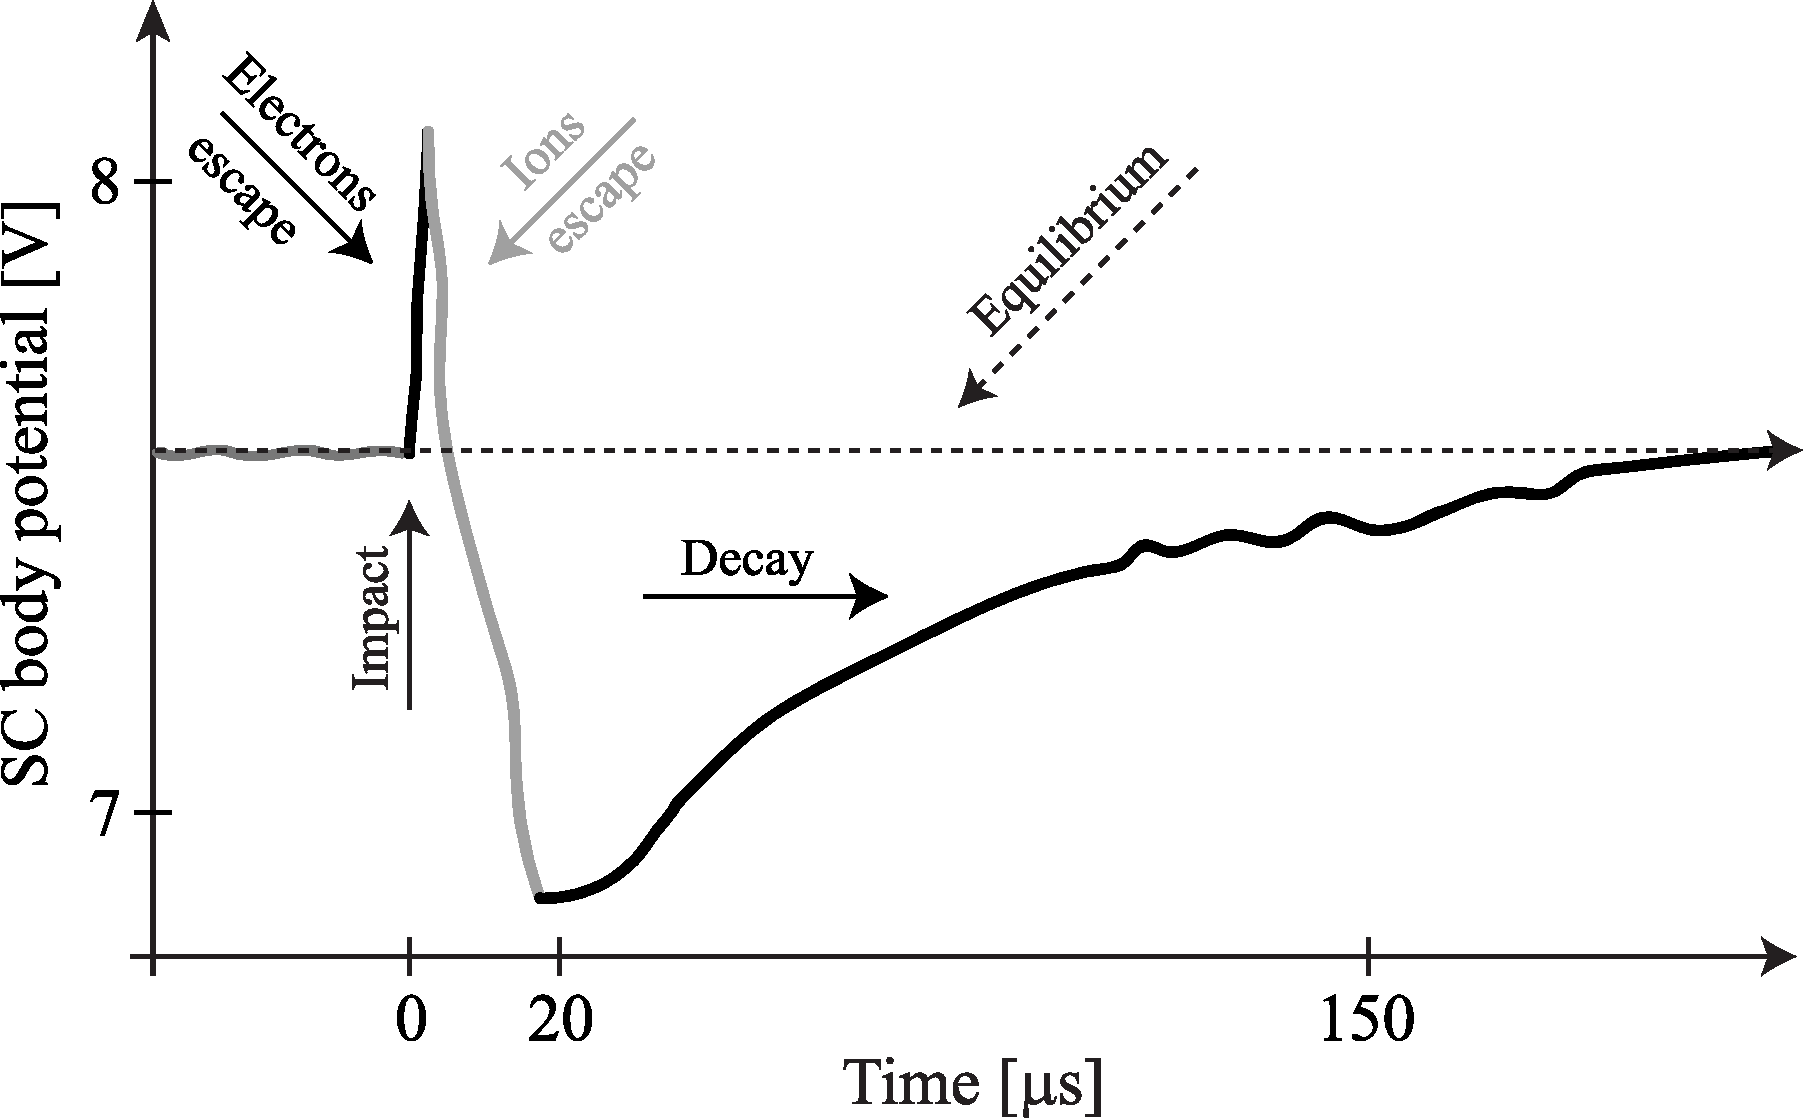
\includegraphics[width=8cm]{figures/impact_wf_gs.pdf}
 	\caption{A simplified dust impact monopole electrical signature after an impact onto a positively charged spacecraft body.}
 	\label{fig:impact_process}
\end{figure}

Therefore, there are several features to look for in the time-domain measurements, such as the quick rise of the signal, and the exponential decay of the maximum. Visual identification is robust to the extent to which experts' opinions on the impact shape agree. Such identification is however very time consuming, and for any reasonably big data set, it is clearly not feasible to use this method alone.

\subsubsection{Hard-coded identification}

The features of dust impact signatures can be translated into algorithmic criteria, which are then efficiently applied to a big data set. While these identification criteria work reasonably well for textbook examples of dust impacts, the actual impacts in space may be quite different from the basic example, as they might contain a lot of noise, saturated data, solitary waves, or a superposition of a dust impact and a wave, and other non-standard signals \citep{vaverka2018comparison,ye2019understanding,malaspina2023dust}. One such algorithm is used for on-board identification of dust impacts on Solar Orbiter \cite{maksimovic2020solar}, and in Paper I, we found this algorithm to be $\SI{94}{\%}$ sensitive and $\SI{79}{\%}$ specific on a sample containing $\SI{50}{\%}$ dust and $\SI{50}{\%}$ non-dust recordings, which was the main motivation for the development of a more reliable automatic identification procedure of that paper. 

\subsubsection{Machine learning}

A supervised machine learning has established itself as a method of time-series classification, particularly in cases, when the exact classification criteria are hard to formulate, but labelled date are abundant \citep{wickstrom2022mixing}. This is a good fit for the problem of dust identification. Methods are available, such as \textit{support vector machine} (SVM), which evaluates a set of pre-defined quantitative features on labelled data, and creates a decision algorithm based on them \citep{vapnik1997support}. \textit{Convolutional neural network} (CNN) is a type of a neural network very useful for the classification of labelled grid-like objects \citep{gu2018recent}. Unlike SVMs, CNNs yield the features vector by convolution operations, and therefore, they don't require a defined feature extracting algorithms. One common disadvantage of CNNs is that they might be difficult to explain, as neural networks generally act like black-boxes, with their internal working hard to interpret. However, great progress was achieved, at least for a limited class of CNNs, in the recent past \citep{samek2021explaining}. If designed to be so, CNN can be explainable to the extent that even features with non-linear effects are interpretable. This not only mitigates the black-box trust issue, but also provides more insight into the problem at hand. In Paper I, both an SVM and an explainable CNN were successfully used to meaningfully improve the performance of the dust identification algorithm, compared to the on-board hard-coded one.

\section{Dust detection flux modelling}

With antenna detection of dust, the whole body of the spacecraft acts as a detection surface for collision between dust grains and the spacecraft. Assuming a 6D phase space probability density function $f(\vec{r},\vec{v})$ for the dust cloud, where $\vec{r}$ is the location and $\vec{v}$ is the velocity of the dust, and normalized to dust number density $n$ as
\begin{equation}
    n(\vec{r}) = \iiint_{\mathbb{R}^3} f(\vec{r},\vec{v}) \,dv_x\,dv_y\,dv_z,
\end{equation}
and a spherical spacecraft with the cross section of $S$, the detection rate $\lambda$ is
\begin{equation}
    \lambda = S \iiint_{\mathbb{R}^3} |\vec{v}-\vec{v}_{sc}| f(\vec{r},\vec{v})  \,dv_x\,dv_y\,dv_z, \label{eq:phase_space_lambda}
\end{equation}
assuming the spacecraft speed $\vec{v}_{sc}$. If the spacecraft moves through a dust cloud with a sharp relative speed between the spacecraft and the dust $v=|\vec{v}_{sc}-\vec{v}|$, the detection rate simplifies to  
\begin{equation}
    \lambda = S n v,
\end{equation}
assuming that the local number density of dust is $n$ and that all the grains are detected, if collided with. In reality, all the collision are never registered, and the higher relative speed $v$ implies a higher charge produced on impact (Eq. \ref{eq:charge_generation}), and in turn higher probability of detection, therefore the rate is sometimes modelled as
\begin{equation}
    \lambda = S n v^{1+\alpha \delta}, \label{eq:rate_semi_general}
\end{equation}
where $\alpha$ is the parameter in charge generation Eq. \ref{eq:charge_generation}, and $\delta$ is the mass distribution slope from Eq. \ref{eq:mass_distribution}. Eq. \ref{eq:rate_semi_general} can be specialized for different dust populations. For example, there is a bond between $\vec{v}_{dust}$ and $r$ for bound dust \citep{szalay2020near}, while $\vec{v}_{dust}$ can be reasonably assumed constant \citep{zaslavsky2021first} for $\beta$ meteoroids, sufficiently far from the Sun. There is also a bond between the number density $n$ and the distance from the Sun for bound dust (Eq. \ref{eq:dust_number_density}) and for $\beta$ meteoroids \ref{eq:beta_number_density}. The number density $n$ and velocity $\vec{v}_{dust}$ of interstellar dust is sometimes assumed constant in space and time. In principle, the cross section $S$ is orientation dependent for non-spherical spacecraft. The total model rate $\Lambda$ in a multi-component model is a superposition of the detection rates $\lambda_i$ for each of the modelled populations as
\begin{equation}
    \Lambda = \sum_{\forall i} \lambda_i,
\end{equation}
where each individual $\lambda_i$ is reasonably approximated. 

Explaining the flux observed on Solar Orbiter with a two component, semi-empirical model, was the goal of Paper II, where we were able to constrain some of the physical parameters of the $\beta$ meteoroids. Building a physics based model for bound dust detections on Parker Solar Probe based on a phase space distribution approach (Eq. \ref{eq:phase_space_lambda}) was the goal of Paper IV and allowed for constraining some of the orbital parameters of the near-solar dust. 

\subsection{Orbital parameters and the data set}

Depending on the orbit of a spacecraft, the observed dust flux is dependent on, and therefore holds the information about different dust populations, while being unable to resolve other populations. We discussed the defining properties of common dust populations in Ch. \ref{ch:populations}. The orbits of selected spacecraft are shown in Fig. \ref{fig:sc_orbits}. In this section, we present different spacecraft, and we explain why their measurements complement each other.  

\begin{figure}[h]
 	\centering
 	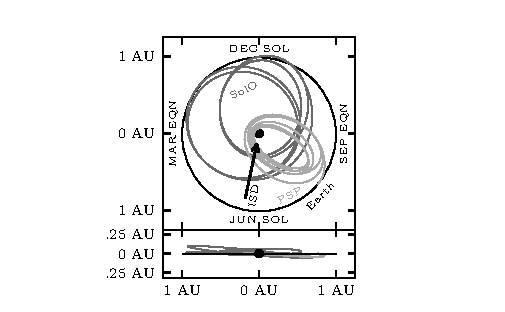
\includegraphics[width=14cm]{figures/solo_orbit.pdf}
 	\caption{The orbit of SolO and PSP in heliocentric (HAE) coordinates between their respective launch date and the summer of 2024, shown in \textit{XY} (top) and \textit{XZ} (bottom) planes. The orbit of the Earth is shown for reference, which is very similar to the orbits of the two STEREO spacecraft. The direction of ISD flow is shown with an arrow.}
 	\label{fig:sc_orbits}
\end{figure}

\subsubsection{Solar Terrestrial Relations Observatory}

The two Solar Terrestrial Relations Observatory (\textit{STEREO}) spacecraft orbit the Sun on a nearly circular orbit close to $\SI{1}{AU}$. Their electrical antenna measurements allow for dust identification \citep{meyer2009dust}. Beyond the intermittent and hard to explain nanodust \citep{meyer2009dust}, the flux was found to be dominated by $\beta$ meteoroids \citep{zaslavsky2012interplanetary}. However, distinguishing $\beta$ meteoroids from bound dust is virtually impossible, since, owing to the circular orbit, the flux of both is expected constant throughout the orbit and the years. This is also an advantage for the detection of interstellar dust (ISD), which is directional, and even though its flux is relatively low, compared to $\beta$ meteoroids, it causes most of the observed variance \citep{zaslavsky2012interplanetary,malaspina2015revisiting,babic2022situ}, with the flux maxima coinciding with the anti-parallel velocity between STEREO and ISD, and minima coinciding with the parallel configuration. Spacecraft located in Earth's L1 point are in just as good position to investigate ISD \citep{malaspina2014interplanetary,malaspina2016database}.

\subsubsection{Solar Orbiter}

SolO orbits the Sun on an elliptical orbit between $\SI{0.3}{AU}$ and $\SI{1}{AU}$ (eccentricity $e \approx 0.52$ in 2024), which means that neither its exposure to bound dust, nor $\beta$ meteoroids is constant. This makes identification of ISD difficult, as it is no longer responsible for an important part of the observed variance. However, the $\beta$ meteoroids are clearly apparent, since the spacecraft's radial speed alternates between negative (pre-perihelia) and positive (post-perihelia), which greatly changes the incidence between the spacecraft and the outgoing $\beta$ meteoroids. Asymmetry in the flux between the inbound and the outbound leg allowed for some of the $\beta$ meteoroid parameters to be constrained by \citet{zaslavsky2021first} and in Paper II. The $\beta$ meteoroids are dominant in the SolO data to the extent that it is not even clear from SolO data alone that bound dust is needed to explain the observed flux.

\subsubsection{Parker Solar Probe}

The orbit of PSP is even more eccentric ($e \approx 0.86$ in 2024), compared to SolO, but even more importantly, PSP gets as close as $\SI{0.052}{AU}$ from the Sun. The relative speed between PSP and the dust components was evaluated by \citet{szalay2020near}, and all suggests that unlike for any other spacecraft, the near-solar dust flux is dominated by bound dust impacts, especially in the post-perihelia. While ISD is difficult to distinguish in SolO data, it is very unlikely to be condifently identified in PSP data, since the variation of the flux on PSP is even much higher, and the alignment is even more unfortunate, with the peak of ISD impacts being nearly aligned with the perihelia (see Fig. \ref{fig:sc_orbits}). The bound dust component, crucial for the flux modelling on PSP, was modelled and constrained in Paper IV. The great eccentricity of PSP poses additional challenges do dust detection, as the electric potential, and even conductivity of the spacecraft changes throughout each orbit significantly, which we also investigated and discussed in Paper IV.

\subsection{Compatibility of Solar Orbiter and Parker Solar Probe dust data}

In Paper II, we presented a Bayesian fit of a semi empirical dust flux model to the SolO data from between 07/2020 and 12/2021. In this section, we present a similar fit to the aggregated PSP data from between 

TBD somewhere here do the plot of PSP and SolO flux







